% !TeX root = construct.tex

\selectlanguage{hebrew}

\chapter{אני מסתפק בסרגל )ועוד משהו(}

%%%%%%%%%%%%%%%%%%%%%%%%%%%%%%%%%%%%%%%%%%%%%%%%%%%%%%%%%%%%%%%

\section{%
מבוא
}\label{s.intro}

כל בנייה בסרגל ומחוגה ניתנת לבנייה עם מחוגה בלבד. משפט זה הוכח בשנת 
$1672$
על ידי
\L{Georg Mohr}
וב-
$1797$
על ידי
\L{Lorenzo Mascheroni}.
נשאלת השאלה: האם כל בנייה בסגל ומחוגה ניתנת לבנייה עם סרגל בלבד? התשובה היא שלילית. ב-
$1822$
המתיטיקאי הצרפתי
\L{Jean-Victor Poncelet}
שיער שכן ניתן להסתפק בסרגל בלבד, בתנאי שקיים במישור מעגל
\textbf{%
אחד%
}.
המשפט הוכח ב-
$1833$
על ידי המתימטיקאי השוויצרי
\L{Jakob Steiner}.

במסמך זה אביא את הוכחת המשפט המבוססת על ההוכחה שמופיעה כבעייה
$34$
ב-%
\L{\cite{dorrie1}},
ועובדה על ידי
\L{Michael Woltermann} \L{\cite{dorrie2}}.%
\footnote{%
ברצוני להודות לו על הרשות להתשמש בעבודתו.
}

%%%%%%%%%%%%%%%%%%%%%%%%%%%%%%%%%%%%%%%%%%%%%%%%%%%%%%%%%%%%%%%


במאה ה-
$19$
הוכח שאם נתחיל עם קטע קו שאורכו 
$1$
)המידות לא משנות, פשוט קובעים שאורך הקטע הוא אחד(, ניתן לבנות קטעי קו באורכים המתקבלים מהמספרים הרציונליים על ידי פעולות החשבון 
$+,-,\times,\div$
ועוד פעולת שורש ריבועי 
$\rule[-5pt]{0pt}{20pt}\sqrt{}$,
\textbf{%
ורק%
}
מספרים אלה.

משפט זה מסביר למה לא ניתן לפתור את הבעיות המפורסמות שהציגו היוונים: חלוקת זווית לשלושה חלקים שווים, בניית קוביה שנפחו פי שניים מהנפח של קוביה נתונה, ובניית ריבוע ששטחו שווה לשטח של מעגל נתון. שתי הבניות הראשונות מחייבות בניית קטע קו שאורכו שורש שלישי של קו אחר, וריבוע המעגל מחייב בניית קטע באורך
$\pi$
שהוא מספר "טרנסנדנטלי", כלומר, אי אפשר לחשב אותו מהמספרים הרציונליים ועוד פעולה שורש מחזקה כלשהי.

עם סרגל בלבד ניתן למצוא את נקודת החיתוך של שני קווים, פעולה לשמעשה פותרת משוואה מסדר ראשון, כלומר, אי אפשר לחשב שורש ריבועי. הבנייה של
\L{Poncelet-Steiner}
מראה שאם קיים מעגל אחד, ניתן להשתמש בו כדי לחשב שורש ריבועי וכך לבניות כל בנייה עםf סרגל ומחוגה.

%%%%%%%%%%%%%%%%%%%%%%%%%%%%%%%%%%%%%%%%%%%%%%%%%%%%%%%%%%%%%%%

עיון בבנייה גיאומטרית יגלה שכל צעד הוא אחת משלוש פעולות:
\begin{itemize}
\item
מציאת נקודת החיתוך של שני קווים ישרים.
\item
מציאת נקודות החיתוך של קו ישר עם מעגל.
\item
מציאת נקודות החיתוך של שני מעגלים.
\end{itemize}
ברור שניתן לבצע את הפעולה הראשונה עם סרגל בלבד. עלינו להראות שעבור שתי הפעולות הראשונות ניתן למוצא בנייה שקולה המשתמשת רק בסרגל עם מעגל אחד.

%%%%%%%%%%%%%%%%%%%%%%%%%%%%%%%%%%%%%%%%%%%%%%%%%%%%%%%%%%%%%%%

מה המשמעות של בנייה עם סרגל בלבד? מעגל מוגדר על ידי נקודה
$O$
שהיא מרכז המעגל, וקטע קו באורך
$r$
שאחת מהנקודות הקצה שלה היא
$O$,
קטע המגדיר את הרדיוס. אם נצליח לבנות את הנקודות
$X,Y$
המסומנות בהתרשים שלהלן, נוכל לטעון שהצלחנו לבנות את נקודות החיתוך של מעגל נתון עם קו נתון ושל שני מעגלים. המעגלים מצויירים בקו מקווקוו כי הם לא ממש מפיעים בבנייה. נמשיך להשתמש בסימון זה: המעגל היחיד הנתון יצוייר בקו רגיל, ומעגלים המשמשים רק להדגמת הבנייה והוכחתה יהיו מקווקווים.


\begin{center}
\selectlanguage{english}
\begin{tikzpicture}[scale=.9]
\fill (0,0) node[above right] {$O$} circle[radius=2pt];
\draw[thick,dashed,name path=circle] (0,0) circle[radius=2cm];
\draw (0,0) -- node[left] {$r$} ++(-60:2cm);
\fill (0,0) ++(-60:2cm) circle[radius=2pt];
\draw[name path=line] (-3,-.5) -- ++(20:6cm);
\path [name intersections={of=circle and line,by={X,Y}}];
\fill (X) node[above right,xshift=-2pt,yshift=4pt] {$X$} circle[radius=2pt];
\fill (Y) node[above left] {$Y$} circle[radius=2pt];
\begin{scope}[xshift=6cm]
\fill (0,0) node[above right] {$O_1$} circle[radius=2pt];
\fill (3,0) node[above right] {$O_2$} circle[radius=2pt];
\draw[thick,dashed,name path=circle1] (0,0) circle[radius=2cm];
\draw[thick,dashed,name path=circle2] (3,0) circle[radius=2cm];
\draw (0,0) -- node[left] {$r_1$} ++(-70:2cm);
\draw (3,0) -- node[left,below] {$r_2$} ++(-20:2cm);
\fill (0,0) ++(-70:2cm) circle[radius=2pt];
\fill (3,0) ++(-20:2cm) circle[radius=2pt];
\path [name intersections={of=circle1 and circle2,by={X,Y}}];
\fill (X) node[above,yshift=4pt] {$X$} circle[radius=2pt];
\fill (Y) node[below,yshift=-4pt] {$Y$} circle[radius=2pt];
\end{scope}
\end{tikzpicture}
\selectlanguage{hebrew}
\end{center}


%%%%%%%%%%%%%%%%%%%%%%%%%%%%%%%%%%%%%%%%%%%%%%%%%%%%%%%%%%%%%%%


תחילה נביא חמש בניות עזר נחוצות )סעיפים
\L{\ref{s.parallel}--\ref{s.root}}%
(,
ואחר כך נראה איך למצוא נקודות חיתוך של קו עם מעגל )סעיף
\L{\ref{s.line-circle}}%
( ושל שני מעלגים )סעיף
\L{\ref{s.circle-circle}}%
(.
%%%%%%%%%%%%%%%%%%%%%%%%%%%%%%%%%%%%%%%%%%%%%%%%%%%%%%%%%%%%%%%

\section{%
בניית קו המקביל לקו נתון%
}\label{s.parallel}

\textbf{%
נתון קו
$l$
המוגדר על ידי שתי נקודות
$A,B$,
ונקודה 
$P$
)שאיננה על הקו( ניתן לבנות קו דרך
$P$
המקביל ל-
$AB$.%
}

נפריד את הבנייה לשני מקרים:
\begin{itemize}
\item
"קו מכוון": נתון שתי נקודות
$A,B$
על הקו והנקודה 
$M$
\textbf{%
החוצה
}
את
$AB$.
\item
כל קו אחר.
\end{itemize}

\textbf{%
קו מכוון:
}
נבנה קרן הממשיכה את
$AP$,
ונבחר
$S$,
נקודה כלשהי על הקרן מעבר ל-%
$AP$.
נבנה את הקווים
$SB$, $SM$, $BP$.
נסמן ב-%
$O$
את נקודת החיתוך של 
$BP$
עם
$SM$.
נבנה קרן הממשיכה את
$AO$
ונסמן ב-%
$Q$
את החיתוך של הקרן
$AO$
עם
$SB$.
\begin{center}
\selectlanguage{english}
\vspace*{-4pt}
\begin{tikzpicture}
\draw[name path=pq] (-4,0) -- (4,0);
\draw (-2,-2) node[below left] {$A$} coordinate (A) -- (2,-2) node[below right] {$B$} coordinate (B);
\fill (A) circle[radius=2pt];
\fill (B) circle[radius=2pt];
\draw[name path=as] (A) -- ++(50:4cm) node[above] {$S$} coordinate (S);
\fill (S) circle[radius=2pt];
\draw[name path=sb] (S) -- (B);
\path [name intersections={of=pq and as,by={P}}];
\path [name intersections={of=pq and sb,by={Q}}];
\fill (P) node[above left] {$P$} circle[radius=2pt];
\fill (Q) node[above right] {$Q$} circle[radius=2pt];
\draw[name path=pb] (P) -- (B);
\draw[name path=qa] (Q) -- (A);
\path [name intersections={of=pb and qa,by={O}}];
\fill (O) node[right,xshift=2pt] {$O$} circle[radius=2pt];
\fill (0,-2) coordinate (M) node[below right] {$M$} circle[radius=2pt];
\draw (S) -- (M);
\end{tikzpicture}
\vspace*{-4pt}
\selectlanguage{hebrew}
\end{center}
מהתרשים נראה ש-% 
$PQ$
מקביל ל-%
$AB$,
אבל זה בדיוק מה שעלינו להוכיח.

ההוכחה תשתמש במשפט של
\L{Ceva}
שנוכיח בהמשך. לפי המשפט, קיים קשר בין האורכים של קטעים המרכיבים את היקף המשולש:
\[
\frac{AM}{MB}\frac{BQ}{QS}\frac{SP}{PA} = 1
\]
$M$
חוצה את
$AB$
ולכן
$\frac{AM}{MB}=1$.
הגורם הראשון של המכלפה מצטמצם ונקבל את המשוואה:
\begin{equation}
\frac{BQ}{QS}=\frac{PA}{SP}=\frac{AP}{PS}\,.
\end{equation}
נוכיח שהמשולש
$\triangle ABS$
דומה ל-%
$\triangle PQS$,
ולכן הקו
$PQ$
מקביל לקו
$AB$
כי
$\angle ABS = \angle PQS$.
ההוכחה שהמשולשים דומים היא:
\vspace*{-10pt}
\[
\renewcommand*{\arraystretch}{2}
\begin{array}{rcl}
BS&=&BQ+QS\\
\disfrac{BS}{QS}&=&\disfrac{BQ}{QS}+\disfrac{QS}{QS} = \disfrac{BQ}{QS}+1\\
AS&=&AP+PS\\
\disfrac{AS}{PS} &=& \disfrac{AP}{PS} + \disfrac{PS}{PS} = \disfrac{AP}{PS} + 1\\
\disfrac{BS}{QS}&=&\disfrac{AS}{PS}\,,
\end{array}
\]
כאשר המשוואה האחרונה מתקבלת ממשוואה-)1(.

כדי להוכיח את המשפט של
\L{Ceva},
נתבונן בתרשימים שלהן:
\begin{center}
\selectlanguage{english}
\vspace*{-4pt}
\begin{tikzpicture}
\path[name path=pq] (-4,0) -- (4,0);
\draw (-2,-2) node[below left] {$A$} coordinate (A) -- (2,-2) node[below right] {$B$} coordinate (B);
\coordinate (M) at (0,-2);
\draw[name path=as] (A) -- ++(50:4cm) node[above] {$S$} coordinate (S);
\draw[name path=sb] (S) -- (B);
\path [name intersections={of=pq and as,by={P}}];
\path [name intersections={of=pq and sb,by={Q}}];
\path[name path=pb] (P) -- (B);
\path[name path=qa] (Q) -- (A);
\path [name intersections={of=pb and qa,by={O}}];
\draw[fill=gray!40] (B) -- (O) -- (Q);
\draw[fill=gray!70] (S) -- (O) -- (Q);
\draw (B) -- (O) -- (A);
\draw (S) -- (O) -- (A);
\draw (A) -- (B) -- (S) -- cycle;
\draw (S) -- (O);
\draw (B) -- (O);
\fill (A) circle[radius=2pt];
\fill (B) circle[radius=2pt];
\fill (S) circle[radius=2pt];
\fill (Q) node[above right] {$Q$} circle[radius=2pt];
\fill (O) node[above left] {$O$} circle[radius=2pt];
\path[name path=al1] (O) -- ($(Q)!(O)!(B)$);
\path [name intersections={of=al1 and sb,by={A1}}];
\draw[thick,dashed] (O) -- (A1);
\begin{scope}[xshift=6cm]
\path[name path=pq] (-4,0) -- (4,0);
\draw (-2,-2) node[below left] {$A$} coordinate (A) -- (2,-2) node[below right] {$B$} coordinate (B);
\coordinate (M) at (0,-2);
\draw[name path=as] (A) -- ++(50:4cm) node[above] {$S$} coordinate (S);
\draw[name path=sb] (S) -- (B);
\path [name intersections={of=pq and as,by={P}}];
\path [name intersections={of=pq and sb,by={Q}}];
\draw[name path=pb] (P) -- (B);
\draw[name path=qa] (Q) -- (A);
\path [name intersections={of=pb and qa,by={O}}];
\draw (B) -- (O) -- (Q);
\draw (A) -- (Q) -- (B);
\draw[fill=gray!40] (B) -- (Q) -- (A);
\draw[fill=gray!70] (S) -- (Q) -- (A);
\draw (A) -- (B) -- (S) -- cycle;
\draw (S) -- (O);
\draw (B) -- (O);
\fill (A) circle[radius=2pt];
\fill (B) circle[radius=2pt];
\fill (S) circle[radius=2pt];
\fill (Q) node[above right] {$Q$} circle[radius=2pt];
\fill (O) node[above left] {$O$} circle[radius=2pt];
\path[name path=al2] (A) -- ($(Q)!(A)!(B)$);
\path [name intersections={of=al2 and sb,by={A2}}];
\draw[thick,dashed] (A) -- (A2);
\end{scope}
\end{tikzpicture}
\vspace*{-6pt}
\selectlanguage{hebrew}
\end{center}
אם הגבהים של שני משולשים שוואים, יחס השטחים שווה ליחס הבסיסים:
\[
A_1 = \frac{1}{2}hb_1,\quad A_2 = \frac{1}{2}hb_2, \quad \frac{A_1}{A_2}=\frac{b_1}{b_2}\,.
\]
בכל אחד מהתרשימים, הגבהים של זוג המשולשים המסומנים באפור שווים. לכן:%
\footnote{%
נשתמש בשם המשולש כקיצור לשטחו.%
}
\[\frac{\triangle BQO}{\triangle SQO} = \frac{BQ}{QS}\;,\quad\quad \frac{\triangle BQA}{\triangle SQA} = \frac{BQ}{QS}\;.
\]
על ידי חיסור של המשולשים המסומנים, נקבל יחס בין המשולשים המסומנים באפור:
\begin{center}
\selectlanguage{english}
\vspace*{-4pt}
\begin{tikzpicture}
\path[name path=pq] (-4,0) -- (4,0);
\draw (-2,-2) node[below left] {$A$} coordinate (A) -- (2,-2) node[below right] {$B$} coordinate (B);
\coordinate (M) at (0,-2);
\draw[name path=as] (A) -- ++(50:4cm) node[above] {$S$} coordinate (S);
\draw[name path=sb] (S) -- (B);
\path [name intersections={of=pq and as,by={P}}];
\path [name intersections={of=pq and sb,by={Q}}];
\path[name path=pb] (P) -- (B);
\draw[thick,name path=qa] (Q) -- (A);
\path [name intersections={of=pb and qa,by={O}}];
\draw[fill=gray!50] (B) -- (O) -- (A);
\draw[fill=gray!70] (S) -- (O) -- (A);
\draw (B) -- (O) -- (A);
\draw (S) -- (O) -- (A);
\draw (A) -- (B) -- (S) -- cycle;
\draw (S) -- (O);
\draw (B) -- (O);
\fill (A) circle[radius=2pt];
\fill (B) circle[radius=2pt];
\fill (S) circle[radius=2pt];
\fill (Q) node[above right] {$Q$} circle[radius=2pt];
\fill (O) node[right,xshift=2pt] {$O$} circle[radius=2pt];
\end{tikzpicture}
\vspace*{-4pt}
\selectlanguage{hebrew}
\end{center}
\[
\frac{BQ}{QS} = \frac{\triangle BQA - \triangle BQO}{\triangle SQA-\triangle SQO} = \frac{\triangle BOA}{\triangle SOA}\,.
\]
החישוב עלול להיראות חשוד. נסביר אותו תוך שימוש בסימונים פשוטים יותר:
\[
\renewcommand*{\arraystretch}{1.6}
\begin{array}{rcl}
 \disfrac{c}{d} &=&\disfrac{a}{b}\\
 \disfrac{e}{f} &=&\disfrac{a}{b}\\
c-e &=& \disfrac{ad}{b} - \disfrac{af}{b}\\
c-e &=& \disfrac{a}{b}(d-f)\\
\disfrac{c-e}{d-f} &=& \disfrac{a}{b}\,.
\end{array}
\]
באופן דומה ניתן להוכיח:
\[
\frac{AM}{MB} = \frac{\triangle AOS}{\triangle BOS}\;,\quad\quad \frac{SP}{PA} =\frac{\triangle SOB}{\triangle AOB}\;,
\]
ומכאן
\[
\frac{AM}{MB}\frac{BQ}{QS}\frac{SP}{PA} = \frac{\triangle AOS}{\triangle BOS}\frac{\triangle BOA}{\triangle SOA}\frac{\triangle SOB}{\triangle AOB}=1\,,
\]
כי השטחים במונה ובמכנה מצטצמים )זכרו שסדר הקודקים במשלוש לא חשוב(.
%%%%%%%%%%%%%%%%%%%%%%%%%%%%%%%%%%%%%%%%%%%%%%%%%%%%%%%%%%%%%%%

\textbf{%
כל קו אחר:
}
נסמן את הקו ב-%
$l$,
נסמן ב-%
$c$
את
\textbf{%
המעגל הקבוע%
}
שמרכזו בנקודה
$O$
והרדיוס שלו הוא קטע קו באורך
$r$,
ונסמן ב-%
$P$
את הנקודה שלא נמצאת על הקו. עליך להשתכנע שהבנייה, כאן ובהמשך, לא תלוייה במיקום המעגל במישור או ברדיוס שלו.

נבחר 
$M$,
נקודה כלשהי על הקו 
$l$,
ונבנה קרן הממשיכה את
$MO$
והחותך את המעגל ב-%
$X,Y$.
\begin{center}
\selectlanguage{english}
\begin{tikzpicture}[scale=.8]
\coordinate (O) at (0,0);
\fill (O) node[below right] {$O$} circle[radius=2pt];
\draw[name path=circle] (O) circle[radius=2cm];
\draw[name path=l] (-4,-3) -- node[above, near end] {$l$} +(9,0);
\path[name path=mo] (-2,-3) coordinate (M) -- ($(-2,-3)!1.65!(O)$);
\fill (M) node[below] {$M$} circle[radius=2pt];
\path [name intersections={of=circle and mo,by={V,U}}];
\fill (U) node[below,xshift=2pt,yshift=-4pt] {$U$} circle[radius=2pt];
\fill (V) node[right,xshift=4pt] {$V$} circle[radius=2pt];
\draw (M) -- (V);
\node at (-1.6,1.6) {$c$};
\fill (-4,1) node[above left] {$P$} circle[radius=2pt];
\end{tikzpicture}
\vspace*{-8pt}
\selectlanguage{hebrew}
\end{center}
קו זה הוא
\textbf{%
קו מכוון%
}
כי 
$O$,
מרכז המעגל, חוצה את הקוטר
$UV$.
נבחר נקודה שנייה 
$A$
על 
$l$
ונשתמש בבבנייה עבור קו מכוון כדי לבנות קו המקביל ל-%
$UV$.
הקו חותך את המעגל
$X,Y$.
\begin{center}
\selectlanguage{english}
\begin{tikzpicture}[scale=.8]
\coordinate (O) at (0,0);
\fill (O) node[below right] {$O$} circle[radius=2pt];
\draw[name path=circle] (O) circle[radius=2cm];
\draw[name path=l] (-4,-3) -- node[above,near end,xshift=24pt] {$l$} +(9,0);
\path[name path=mo] (-2,-3) coordinate (M) -- ($(-2,-3)!1.65!(O)$);
\fill (M) node[below] {$M$} circle[radius=2pt];
\path [name intersections={of=circle and mo,by={V,U}}];
\fill (U) node[below,xshift=2pt,yshift=-4pt] {$U$} circle[radius=2pt];
\fill (V) node[right,xshift=4pt] {$V$} circle[radius=2pt];
\draw (M) -- (V);
\path[name path=ax] (-3,-3) coordinate (A) -- ($(-3,-3)!1.8!(-1,0)$);
\fill (A) node[below] {$A$} circle[radius=2pt];
\path [name intersections={of=circle and ax,by={Y,X}}];
\fill (X) node[left] {$X$} circle[radius=2pt];
\fill (Y) node[above] {$Y$} circle[radius=2pt];
\node at (-1.6,1.6) {$c$};
\draw (A) -- (Y);
\fill (-4,1) node[above left] {$P$} circle[radius=2pt];
\end{tikzpicture}
\vspace*{-6pt}
\selectlanguage{hebrew}
\end{center}
נבנה קוטר
$XX'$
וקוטר
$YY'$.
נבנה קרן מ-%
$X'Y'$
ונסמן ב-%
$B$,
את נקודת החיתוך עם 
$l$.
\begin{center}
\selectlanguage{english}
\begin{tikzpicture}[scale=.8]
\coordinate (O) at (0,0);
\fill (O) node[below right] {$O$} circle[radius=2pt];
\draw[name path=circle] (O) circle[radius=2cm];
\draw[name path=l] (-4,-3) -- node[above,near end,xshift=24pt] {$l$} +(9,0);
\path[name path=mo] (-2,-3) coordinate (M) -- ($(-2,-3)!1.65!(O)$);
\fill (M) node[below] {$M$} circle[radius=2pt];
\path [name intersections={of=circle and mo,by={V,U}}];
\fill (U) node[below,xshift=2pt,yshift=-4pt] {$U$} circle[radius=2pt];
\fill (V) node[right,xshift=4pt] {$V$} circle[radius=2pt];
\draw (M) -- (V);
\path[name path=ax] (-3,-3) coordinate (A) -- ($(-3,-3)!1.8!(-1,0)$);
\fill (A) node[below] {$A$} circle[radius=2pt];
\path [name intersections={of=circle and ax,by={Y,X}}];
\fill (X) node[left] {$X$} circle[radius=2pt];
\fill (Y) node[above] {$Y$} circle[radius=2pt];
\node at (-1.6,1.6) {$c$};
\draw (A) -- (Y);
\fill (-4,1) node[above left] {$P$} circle[radius=2pt];
\path[name path=xo] (X) -- ($(X)!2.2!(O)$);
\path[name intersections={of=circle and xo,by={Xp}}];
\fill (Xp) node[right,xshift=2pt,yshift=-2pt] {$X'$} circle[radius=2pt];
\draw (X) -- (Xp);
\path[name path=yo] (Y) -- ($(Y)!2.2!(O)$);
\path[name intersections={of=circle and yo,by={y,Yp}}];
\fill (Yp) node[below right] {$Y'$} circle[radius=2pt];
\draw (Y) -- (Yp);
\path[name path=xy] (Xp) -- ($(Xp)!1.6!(Yp)$);
\path[name intersections={of=l and xy,by={B}}];
\fill (B) node[below] {$B$} circle[radius=2pt];
\draw (Xp) -- (B);
\draw[thick,dashed,name path=z] (-4,0) -- (4,0) node[above,near end,xshift=40pt] {$l'$};
\path[name intersections={of=ax and z,by={Z}}];
\path[name intersections={of=xy and z,by={Zp}}];
\fill (Z) node[above left] {$Z$} circle[radius=2pt];
\fill (Zp) node[below right] {$Z'$} circle[radius=2pt];
\end{tikzpicture}
\vspace*{-10pt}
\selectlanguage{hebrew}
\end{center}
\textbf{%
טענה:%
}
$l$
הוא
\textbf{%
קו מכוון%
}
כי
$M$
חוצה את
$AB$.

מהטענה אפשר לבנות קו דרך 
$P$
מקביל ל-%
$AB$
לפי הבנייה עבור קו מכוון.

\textbf{%
הוכחה:%
}
$OX,OX',OY,OY'$
הם כולם רדיוסים של המעגל, ו-%
$\angle XOY = \angle X'OY'$
כי הן זוויות נגדיות. לכן,
$\triangle XOY$
חופף ל-%
$\triangle X'OY'$
לפי צלע-זווית-צלע. נגדיר
$l'$,
קו מקביל ל-%
$l$,
החותך את 
$XY$
ב-%
$Z$
והחותך את 
$X',Y'$
ב-%
$Z'$.
$\triangle XOZ$,
$\triangle X'OZ'$
חופפים לפי זווית-צלע-זווית, ולכן
$ZO=OZ'$. 
הוכחנו ש-%
$AMOZ$
ו-%
$BMOZ'$
מקביליות, ולכן
$AM=ZO=OZ'=MB$.

\textbf{%
מסקנה:%
}
נתון קטע קו 
$AB$
ונקודה
$P$
שאיננה על הקו. ניתן לבנות קטע קו
$PQ$
המקביל ל-%
$AB$,
שאורכו שווה לאורכו של
$AB$.
במילים אחרות: ניתן להעתיק את
$AB$
מקביל לעצמו כך שקצה אחד יהיה נקודה כלשהי
$P$.

\textbf{%
הוכחה:%
}
בסעיף זה הוכחנו שניתן לבנות קו 
$m$
דרך 
$P$
המקביל ל-%
$AB$,
וקו
$n$
דרך 
$B$
המקביל ל-%
$AP$.
המרובע 
$ABQP$
הוא מקבילית, ולכן הצלעות הנגדיות שוות:
$AB=PQ$.
\begin{center}
\selectlanguage{english}
\begin{tikzpicture}[scale=.8]
\coordinate (P) at (0,0);
\coordinate (Q) at (3,0);
\coordinate (A) at (-2,2.5);
\coordinate (B) at (1,2.5);
\draw ($(P)!-.6!(Q)$) -- node[above,near end,xshift=36pt] {$m$} ($(P)!1.8!(Q)$);
\fill (P) node[below] {$P$} circle[radius=2pt];
\fill (Q) node[below left] {$Q$} circle[radius=2pt];
\draw ($(A)!-.6!(B)$) -- node[above,near end,xshift=40pt] {$l$} ($(A)!2.5!(B)$);
\fill (A) node[above left] {$A$} circle[radius=2pt];
\fill (B) node[above right] {$B$} circle[radius=2pt];
\draw (A) -- (P);
\draw ($(B)!-.3!(Q)$) -- node[above,near end,xshift=24pt,yshift=-24pt] {$n$} ($(B)!1.4!(Q)$);
\end{tikzpicture}
\selectlanguage{hebrew}
\end{center}

%%%%%%%%%%%%%%%%%%%%%%%%%%%%%%%%%%%%%%%%%%%%%%%%%%%%%%%%%%%%%%%

\section{%
בניית אנח לקו נתון%
}\label{s.perpendicular}

\textbf{%
נתון קו
$l$
ונקודה
$P$
)שאיננה על הקו( ניתן לבנות אנח ל-%
$l$
דרך
$P$.%
}

נבנה )לפי סעיף
\L{\ref{s.parallel}}(
קו
$l'$
מקביל ל-%
$l$
החותך את
\textbf{%
המעגל הקבוע%
}
ב-%
$U,V$.
נבנה את הקוטר
$UOU'$
והמיתר
$U'V$.
\begin{center}
\selectlanguage{english}
\begin{tikzpicture}[scale=.8]
\coordinate (O) at (0,0);
\coordinate (P) at (3.5,.6);
\node at (-1.6,1.6) {$c$};
\draw[name path=circle] (O) circle[radius=2cm];
\draw[name path=l] (-4,-3) -- node[above,near end,xshift=45pt] {$l$} ++(9.5,0);
\draw[name path=lp] (-3,-1) -- node[above,near end,xshift=45pt] {$l'$} ++(7.5,0);
\fill (O) node[above left] {$O$} circle[radius=2pt];
\fill (P) node[right] {$P$} circle[radius=2pt];
\path[name intersections={of=circle and lp,by={U,V}}];
\fill (U) node[below left] {$U$} circle[radius=2pt];
\fill (V) node[below right] {$V$} circle[radius=2pt];
\path[name path=d] (U) -- ($(U)!2.3!(O)$);
\path[name intersections={of=circle and d,by={Up}}];
\draw (U) -- (Up);
\fill (Up) node[above right] {$U'$} circle[radius=2pt];
\draw (Up) -- (V);
\path[name path=p] (P) -- ++(0,-4);
\draw[name intersections={of=p and l,by={X}}];
\fill (X) circle[radius=2pt];
\draw[thick,dashed] (P) -- (X);
\draw ($(U)!.9!(V)$) -- ++(0,.3) -| (V);
\end{tikzpicture}
\vspace*{-8pt}
\selectlanguage{hebrew}
\end{center}
$\angle UVU'$
היא זווית ישרה כי היא נשענת על מחצית המעגל. מכאן ש-%
$U'V$
הוא אנח ל-%
$UV$
ו-%
$l'$.
נבנה קו מקביל ל-%
$U'V$
 דרך 
$P$
)לפי סעיף
\L{\ref{s.parallel}}(.



%%%%%%%%%%%%%%%%%%%%%%%%%%%%%%%%%%%%%%%%%%%%%%%%%%%%%%%%%%%%%%%

\section{%
העתקת קטע קו נתון בכיוון נתון%
}\label{s.direction}

\textbf{%
נתון נקודה
$A$,
קטע קו
$PQ$
וכיוון, ניתן לבנות קטע קו
$AS$
כך ש-%
$AS=PQ$.%
}

המסקנה בסוף סעיף
\L{\ref{s.parallel}}
מראה שאפשר להעתיק קטע קו מקביל לעצמו. כאן נוכיח שניתן להנתיק קטע קו בכיוון של כל קו אחר. הכוונה של "כיוון" היא שקו המוגדר על ידי שתי נקודות
$A',H'$
מגדיר זווית
$\theta$
יחסית לציר כלשהו. המשימה היא להעתיק את קטע הקו
$PQ$
ל-%
$AS$,
כך ש-%
$AS$
יהיה באותה זווית
$\theta$
יחסית לאותו ציר. בתרשים הציר הוא הכיוון של 
$PQ$
אבל אין לזה חשיבות.
\begin{center}
\selectlanguage{english}
\vspace*{-8pt}
\begin{tikzpicture}[scale=.8]
\coordinate (A) at (0,0);
\coordinate (P) at (1,-1.5);
\coordinate (Q) at (2.5,-1.5);
\draw (P) -- (Q);
\fill (P) node[left] {$P$} circle[radius=2pt];
\fill (Q) node[right] {$Q$} circle[radius=2pt];
\coordinate (A1) at (-3,1);
\draw (A1) -- ++(60:3cm) coordinate (H1);
\draw[thick,dashed] (A1) -- ++(0:1.5cm);
\fill (A1) node[left] {$A'$} circle[radius=2pt];
\fill (H1) node[left] {$H'$} circle[radius=2pt];
\draw[thick,dashed] (A) -- ++(60:1.5cm);
\draw[thick,dashed] (A) -- ++(1.5,0);
\fill (A) node[left] {$A$} circle[radius=2pt];
\node[above right,xshift=4pt] at (A1) {$\theta$};
\node[above right,xshift=4pt] at (A) {$\theta$};
\end{tikzpicture}
\vspace*{-12pt}
\selectlanguage{hebrew}
\end{center}
נתחיל את הבנייה על ידי העתקת קטע הקו
$A'H'$
אל 
$AH$
כך ש-%
$AH$
יהיה מקביל ל-%
$A'H'$.
הבנייה אפשרית לפי המסקנה בסוף סעיף
\L{\ref{s.parallel}}.
באותו אופן נעתיק את
$PQ$
ל-%
$AK$
כך ש-%
$AK$
מקביל ל-%
$PQ$.
\begin{center}
\selectlanguage{english}
\vspace*{-4pt}
\begin{tikzpicture}[scale=.8]
\coordinate (A) at (0,0);
\coordinate (P) at (1,-1.5);
\coordinate (Q) at (2.5,-1.5);
\draw (P) -- (Q);
\fill (P) node[left] {$P$} circle[radius=2pt];
\fill (Q) node[right] {$Q$} circle[radius=2pt];
\coordinate (A1) at (-3,1);
\draw (A1) -- ++(60:3cm) coordinate (H1);
\draw[thick,dashed] (A1) -- ++(0:1.5cm);
\fill (A1) node[left] {$A'$} circle[radius=2pt];
\fill (H1) node[left] {$H'$} circle[radius=2pt];
\draw (A) -- ++(60:3cm) coordinate (H);
\fill (H) node[left] {$H$} circle[radius=2pt];
\draw (A) -- ++(1.5,0) coordinate (K);
\fill (K) node[below right] {$K$} circle[radius=2pt];
\draw (A) -- (K);
\fill (A) node[left] {$A$} circle[radius=2pt];
\node[above right,xshift=4pt] at (A1) {$\theta$};
\node[above right,xshift=4pt] at (A) {$\theta$};
\end{tikzpicture}
\vspace*{-8pt}
\selectlanguage{hebrew}
\end{center}
הזווית
$\angle HAK$
שווה ל-%
$\theta$,
לכן כל מה שנשאר הוא למצוא נקודה
$S$
על
$AH$
כך ש-%
$AS=AK$.

\textbf{%
במעגל הקבוע%
}
$c$
נבנה שני רדיוסים
$OU$
ו-%
$OV$
מקביליים ל-%
$AH$
ו-%
$AK$,
בהתאמה, ונבנה קרן דרך
$K$
המקבילה ל-%
$UV$.
נסמן את נקודת החיתוך של הקו עם
$AH$
ב-%
$S$.

\textbf{%
טענה:
}
$AS=PQ$.
\begin{center}
\selectlanguage{english}
\begin{tikzpicture}[scale=.8]
\coordinate (A) at (0,0);
\coordinate (P) at (1,-1.5);
\coordinate (Q) at (2.5,-1.5);
\draw (P) -- (Q);
\fill (P) node[left] {$P$} circle[radius=2pt];
\fill (Q) node[right] {$Q$} circle[radius=2pt];
\coordinate (A1) at (-3,1);
\draw (A1) -- ++(60:3cm) coordinate (H1);
\fill (A1) node[left] {$A'$} circle[radius=2pt];
\fill (H1) node[left] {$H'$} circle[radius=2pt];
\draw (A) -- ++(60:3cm) coordinate (H);
\fill (A) node[left] {$A$} circle[radius=2pt];
\fill (H) node[left] {$H$} circle[radius=2pt];
\coordinate (O) at (6,1);
\node at (4.8,3.4) {$c$};
\draw[name path=circle] (O) circle[radius=2.5cm];
\fill (O) node[above left] {$O$} circle[radius=2pt];
\draw (A) -- ++(1.5,0) coordinate (K);
\fill (K) node[below right] {$K$} circle[radius=2pt];
\draw (A) -- (K);
\path[name path=u] (O) -- ++(60:2.5cm);
\path[name path=v] (O) -- ++(2.5,0);
\path[name intersections={of=circle and u,by={U}}];
\path[name intersections={of=circle and v,by={V}}];
\fill (U) node[above right] {$U$} circle[radius=2pt];
\fill (V) node[right] {$V$} circle[radius=2pt];
\draw (O) -- (U) -- (V) -- cycle;
\path (A) -- ++(60:1.5cm) coordinate (S);
\fill (S) node[above left] {$S$} circle[radius=2pt];
\draw (K) -- (S);
\draw[very thick] (A) -- (S);
\node[above right,xshift=4pt] at (A) {$\theta$};
\node[above right,xshift=4pt] at (O) {$\theta$};
\node[above right,xshift=4pt] at (A1) {$\theta$};
\draw[thick,dashed] (A1) -- ++(1.5,0);
\end{tikzpicture}
\vspace*{-4pt}
\selectlanguage{hebrew}
\end{center}
\textbf{%
הוכחה:
}
$AH$
מקביל ל-%
$OU$
ו-%
$AK$
מקביל ל-%
$OV$,
ולכן
$\angle SAK=\angle HAK=\theta=\angle UOV$.
$SK$
מקביל ל-%
$UV$,
והמשולש
$\triangle SAK$
דומה למשולש
$\triangle UOV$
לפי זווית-זווית-זווית.
$\triangle UOV$
הוא משולש שווה שוקיים כי
$OU$, $OV$
הם רדיוסים של אותו מעגל. מכאן,
$\triangle SAK$
הוא משולש שווה שוקיים ו-%
$AS=AK=PQ$.



%%%%%%%%%%%%%%%%%%%%%%%%%%%%%%%%%%%%%%%%%%%%%%%%%%%%%%%%%%%%%%%

\section{%
בניית קטע קו שאורכו מוגדר יחסית לשלושה קטעי קו אחרים%
}\label{s.relative}

\textbf{%
נתון קטעי קו באורכים
$n, m, s$,
ניתן לבנות קטע קו באורך
$x=\disfrac{n}{m}s$.%
}

קטעי הקו הנתונים נמצאים במיקומים כלשהם במישור ובכיוונים כלשהם.
\begin{center}
\selectlanguage{english}
\begin{tikzpicture}[scale=.9]
\draw (0,0) -- node[above] {$s$} ++(30:1.5cm);
\draw (2,1.2) -- node[above] {$m$} ++(-10:2.5cm);
\draw (-2,1.5) -- node[above] {$n$} ++(5:2cm);
\fill (0,0) circle[radius=2pt];
\fill (2,1.2) circle[radius=2pt];
\fill (-2,1.5) circle[radius=2pt];
\fill (0,0) ++(30:1.5cm) circle[radius=2pt];
\fill (2,1.2) ++(-10:2.5cm) circle[radius=2pt];
\fill (-2,1.5) ++(5:2cm) circle[radius=2pt];
\end{tikzpicture}
\vspace*{-8pt}
\selectlanguage{hebrew}
\end{center}
נבחר נקודה כלשהי
$A$
ונבנה שתי קרנות 
$AB,AC$.
לפי סעיף
\L{\ref{s.direction}}
ניתן למצוא נקודות
$M,N,S$
כך ש-%
$AM= m$, $AN =n$
ו-%
$AS=s$.
נבנה דרך
$N$
קו המקביל ל-%
$MS$
החותך את
$AC$
ב-%
$X$,
ונסמן את אורכו ב-%
$x$.
המשולש
$\triangle MAS$
דומה למשולש
$\triangle NAX$
לפי זווית-זווית-זווית, ולכן:
\[
\frac{m}{n}=\frac{s}{x}, \quad\quad x=\disfrac{n}{m}s\,.
\]
\begin{center}
\selectlanguage{english}
\vspace*{-10pt}
\begin{tikzpicture}
\coordinate (A) at (0,0);
\draw[name path=ac] (A) node[left] {$A$} -- ++(7,0) node[right] {$C$};
\draw (A) -- ++(40:5cm) node[right] {$B$};
\fill (A) circle[radius=2pt];
\fill (A) ++(40:5cm) circle[radius=2pt];
\fill (A) ++(7,0) circle[radius=2pt];
\path (A) -- node[above,xshift=-2pt] {$m$} ++(40:3cm) coordinate (M) node[above left] {$M$};
\path (A) -- ++(40:4cm) coordinate (N) node[above left] {$N$};
\fill (M) circle[radius=2pt];
\fill (N) circle[radius=2pt];
\path[name path=ms] (M) -- ++(-50:3.5cm);
\path[name path=nx] (N) -- ++(-50:4cm);
\path[name intersections={of=ac and ms,by={S}}];
\path[name intersections={of=ac and nx,by={X}}];
\fill (S) circle[radius=2pt] node[below] {$S$};
\fill (X) circle[radius=2pt] node[below] {$X$};
\path (A) -- node[below] {$s$} (S);
\draw (S) -- (M);
\draw (X) -- (N);
\node at (7,2.5) {$AN=n$};
\node at (7,2) {$AX=x$};
\end{tikzpicture}
\selectlanguage{hebrew}
\end{center}



%%%%%%%%%%%%%%%%%%%%%%%%%%%%%%%%%%%%%%%%%%%%%%%%%%%%%%%%%%%%%%%

\section{%
בניית שורש ריבועי%
}\label{s.root}

\textbf{%
נתון קטעי קו באורכים
$a,b$,
ניתן לבעות קטע קו שאורכו
$\rule[-5pt]{0pt}{10pt}\sqrt{ab}$.}

אנו שואפים לבטא את
$\rule[-5pt]{0pt}{20pt}x=\sqrt{ab}$
בצורה
$x=\frac{n}{m}s$
כדי להשתמש בבנייה מסעיף
\L{\ref{s.relative}}.
\vspace*{-8pt}
\begin{itemize}
\item עבור
$n$
נשתמש ב-%
$d$,
הקוטר של
\textbf{%
המעגל הקבוע%
}.
\item עבור
$m$
נשתמש ב-%
$t=a+b$
שניתן לבנות מהאורכים הנתונים
$a,b$
לפי סעיף
\L{\ref{s.direction}}.
\item 
נגדיר
$\rule[-5pt]{0pt}{20pt}s=\sqrt{hk}$
כאשר 
$h,k$
מוגדרים כביטויים מעל האורכים
$a,b,t,d$,
ונראה איך ניתן לבנות קטע קו באורך 
$\rule[-5pt]{0pt}{20pt}s=\sqrt{hk}$.
\end{itemize}
נגדיר
$h=\disfrac{d}{t}a$, $k=\disfrac{d}{t}b$,
ונחשב:
\[
x=\sqrt{ab}=\sqrt{\frac{th}{d}\frac{tk}{d}}=\sqrt{\left(\frac{t}{d}\right)^2hk}=\frac{t}{d}hk=\frac{t}{d}s\,.
\]
נחשב גם: 
\[
h+k = \frac{d}{t}a + \frac{d}{t}b = \frac{d(a+b)}{t} = \frac{dt}{t} = d\,.
\]

לפי סעיף
\L{\ref{s.direction}}
ניתן לבנות
$HA= h$
על הקוטר
$HK$
של
\textbf{%
המעגל הקבוע%
}.
מ-%
$h+k=d$, $AK=k$.
\begin{center}
\selectlanguage{english}
\vspace*{-4pt}
\begin{tikzpicture}[scale=.8]
\coordinate (O) at (0,0);
\coordinate (H) at (-3,0);
\coordinate (K) at (3,0);
\node at (-2.4,2.4) {$c$};
\draw (H) -- (K);
\draw[name path=circle] (O) circle[radius=3cm];
\fill (O) node[below] {$O$} circle[radius=2pt];
\fill (H) node[left] {$H$} circle[radius=2pt];
\fill (K) node[right] {$K$} circle[radius=2pt];
\path[name path=as] (1,0) coordinate (A) -- ++(0,3.2);
\fill (A) node[below] {$A$} circle[radius=2pt];
\path[name intersections={of=circle and as,by={S}}];
\fill (S) node[above] {$S$} circle[radius=2pt];
\draw (A) -- node[right,yshift=-6pt] {$\sqrt{hk}$} node[right,near end,yshift=-6pt] {$s=$} (S);
\path (H) -- node[above] {$h$} (A);
\path (A) -- node[above] {$k$} (K);
\draw[thick,dashed] (O) -- node[left] {$\frac{d}{2}$} (S);
\node at (.5,-1.5) {$\frac{d}{2}-k$};
\draw[->] (.5, -1.2) -- ++(0,1);
\draw (.8,0) -- ++(0,.2) -- ++(.2,0);
\end{tikzpicture}
\vspace*{-8pt}
\selectlanguage{hebrew}
\end{center}
לפי סעיף
\L{\ref{s.perpendicular}}
ניתן לבנות דרך
$A$
אנח ל-%
$HK$,
ונסמן ב-%
$S$
את החיתוך של האנח עם
\textbf{%
המעגל הקבוע%
}.
$OS=OK=\frac{d}{2}$
כי הם רדיוסים של המעגל, ו-%
$OA=\frac{d}{2}-k$.
לפי משפט פיתגורס:
\[
\renewcommand*{\arraystretch}{1.6}
\begin{array}{rcl}
SA^2 &=& \left(\disfrac{d}{2}\right)^2 - (\disfrac{d}{2}-k)^2\\
&=& \left(\disfrac{d}{2}\right)^2 - \left(\disfrac{d}{2}\right)^2 + 2\disfrac{dk}{2} - k^2\\
&=& k(d-k)\\
&=& kh,\quad\quad\quad h+k=d\quad \textrm{\R{כי}}\\
s&=&SA=\sqrt{hk}\,.
\end{array}
\]
\vspace*{-8pt}
כעת ניתן לבנות
$x=\disfrac{t}{d}s$
לפי סעיף
\L{\ref{s.relative}}.


%%%%%%%%%%%%%%%%%%%%%%%%%%%%%%%%%%%%%%%%%%%%%%%%%%%%%%%%%%%%%%%

\section{%
בניית נקודות חיתוך של קו עם מעגל%
}\label{s.line-circle}
\textbf{%
נתון קו
$l$
ומעגל
$c$
שמרכזו
$O$
והרדיוס שלו
$r$.
ניתן לבנות את נקודות החיתוך של הקו עם המעגל.%
}

לא מדובר על המעגל הקבוע, אלא על מעגל המוגדר על ידי מרכזו וקטע קו שהוא הרדיוס.
\begin{center}
\selectlanguage{english}
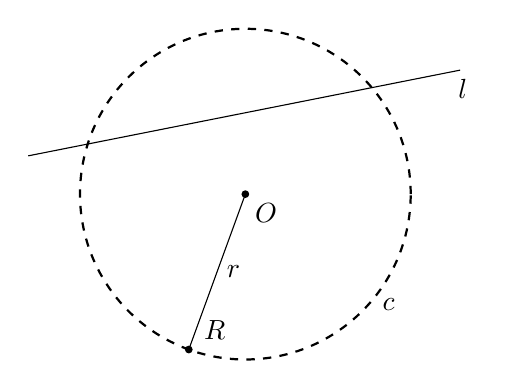
\begin{tikzpicture}[scale=.7]
\coordinate (O) at (0,0);
\node at (2.6,-2) {$c$};
\draw[thick,dashed] (O) circle[radius=3cm];
\fill (O) node[below right] {$O$} circle[radius=2pt];
\draw (O) -- node[right] {$r$} ++(-110:3cm) coordinate (R);
\fill (R) circle[radius=2pt] node[above right,xshift=2pt] {$R$};
\draw (O) +(170:4cm) -- node[below, near end,xshift=40pt,yshift=8pt] {$l$} ++(30:4.5cm);
\end{tikzpicture}
\vspace*{-8pt}
\selectlanguage{hebrew}
\end{center}
לפי סעיף
\L{\ref{s.perpendicular}}
ניתן לבנות אנח ממרכז המעגל
$O$
לקו
$l$.
נסמן ב-%
$M$
את נקודת החיתוך של הקו עם האנח. 
$M$
חוצה של המיתר 
$XY$,
כאשר 
$X,Y$
הן נקודות החיתוך של הקו עם המעגל. שימו לב שבתרשים
$X$, $Y$, $s$
הם רק סימונים. טרם בנינו את נקודות החיתוך.
\begin{center}
\selectlanguage{english}
\begin{tikzpicture}[scale=.7]
\coordinate (O) at (0,0);
\node at (2.6,-2) {$c$};
\draw[thick,dashed,name path=circle] (O) circle[radius=3cm];
\fill (O) node[below right] {$O$} circle[radius=2pt];
\draw (O) -- node[right] {$r$} ++(-110:3cm) coordinate (R);
\fill (R) node[above right,xshift=2pt] {$R$} circle[radius=2pt];
\draw[name path=l] (O) ++(170:4cm) -- node[below, near end,xshift=40pt,yshift=12pt] {$l$} ++(20:8cm);
\path[name intersections={of=circle and l,by={Y,X}}];
\fill (X) node[above left] {$X$} circle[radius=2pt];
\fill (Y) node[above right] {$Y$} circle[radius=2pt];
\draw (O) -- node[below] {$r$} (X);
\path (X) -- ($(X)!.5!(Y)$) coordinate (M);
\fill (M) node[above] {$M$} circle[radius=2pt];
\draw (O) -- node[right] {$t$} (M);
\path (X) -- node[above] {$s$} (M);
\path (M) -- node[above] {$s$} (Y);
\draw (O) ++(170:4cm) -- ++(20:3.1cm) -- ++(-70:10pt) -- ++(20:10pt);
\end{tikzpicture}
\vspace*{-6pt}
\selectlanguage{hebrew}
\end{center}
$\triangle OMX$
הוא מעגל ישר זווית, ולכן
$\rule[-5pt]{0pt}{30pt}s^2=r^2-t^2=\sqrt{(r+t)(r-t)}$.
$r$
נתון כרדיוס המעגל, ו-%
$t$
הוגדר כאורך של
$OM$,
קטע קו שבנינו. לפי סעיף
\L{\ref{s.direction}}
ניתן לבנות קטעי קו באורך
$t$
מהנקודה 
$O$
בשני הכיוונים
$RO$
ו-%
$OR$.
כלומר, ניתן לבנות קטעים באורכים
$r+t,r-t$.
לפי סעיף
\L{\ref{s.root}}
ניתן לבנות קטע קו באורך
$\rule[-5pt]{0pt}{30pt}s=\sqrt{(r+t)(r-t)}$.
שוב לפי סעיף
\L{\ref{s.direction}},
ניתן לבנות קטעי קו באורך 
$s$
על הקו הנתון
$l$
מהנקודה
$M$
בשני הכיוונים. הקצה השני של כל אחד מקטעי הקו האלה הוא נקודת חיתוך של הקו עם המעגל.

%%%%%%%%%%%%%%%%%%%%%%%%%%%%%%%%%%%%%%%%%%%%%%%%%%%%%%%%%%%%%%%

\section{%
בניית נקודות חיתוך של שני מעגלים%
}\label{s.circle-circle}

\textbf{%
נתון שני מעגלים עם מרכזים
$O_1,O_2$
והדיוסים
$r_1,r_2$.
ניתן לבנות את נקודות החיתוך שלהם
$X,Y$%
}

עם סרגל ניתן לבנות את קטע הקו
$O_1O_2$
המחבר את שני המרכזים. נסמן את אורכו ב-%
$t$.
\begin{center}
\selectlanguage{english}
\begin{tikzpicture}[scale=1.1]
\coordinate (O1) at (0,0);
\coordinate (O2) at (2.5,0);
\fill (O1) node[below left] {$O_1$} circle[radius=2pt];
\fill (O2) node[below right] {$O_2$} circle[radius=2pt];
\draw[thick,dashed,name path=circle1] (O1) circle[radius=2cm];
\draw[thick,dashed,name path=circle2] (O2) circle[radius=1.6cm];
\path [name intersections={of=circle1 and circle2,by={X,Y}}];
\draw (O1) -- node[above] {$r_1$} ++(160:2cm);
\draw (O2) -- node[above] {$r_2$} ++(30:1.6cm);
\fill (O1) ++(160:2cm) circle[radius=2pt];
\fill (O2) ++(30:1.6cm) circle[radius=2pt];
\draw (O1) -- (O2);
\node at (-1.7,1.6) {$c_1$};
\node at (3.8,1.4) {$c_2$};
\draw[<->] (0,-1) -- node[fill=white] {$t$} (2.5,-1);
\node at (6,0) {$t=O_1O_2$};
\end{tikzpicture}
\selectlanguage{hebrew}
\end{center}
נסמן ב-%
$A$
את נקודת החיתוך של
$O_1O_2$
עם
$XY$,
ונסמן את האורכים
$q=O_1A,x=XA$.
\begin{center}
\selectlanguage{english}
\begin{tikzpicture}[scale=1.1]
\coordinate (O1) at (0,0);
\coordinate (O2) at (2.5,0);
\fill (O1) node[below left] {$O_1$} circle[radius=2pt];
\fill (O2) node[below right] {$O_2$} circle[radius=2pt];
\draw[thick,dashed,name path=circle1] (O1) circle[radius=2cm];
\draw[thick,dashed,name path=circle2] (O2) circle[radius=1.6cm];
\path [name intersections={of=circle1 and circle2,by={X,Y}}];
\fill (X) node[above,yshift=4pt] {$X$} circle[radius=2pt];
\fill (Y) node[below,yshift=-4pt] {$Y$} circle[radius=2pt];
\draw[thick,dashed] (O1) -- node[above,xshift=-4pt] {$r_1$} (X);
\draw[thick,dashed] (O2) -- node[above,xshift=4pt] {$r_2$} (X);
\draw[name path=oo] (O1) -- (O2);
\node at (-1.7,1.6) {$c_1$};
\node at (3.8,1.4) {$c_2$};
\draw[name path=xy] (X) -- (Y);
\path[name intersections={of=xy and oo,by={A}}];
\fill (A) node[below left] {$A$} circle[radius=2pt];
\path (O1) -- node[below,xshift=-2pt] {$q$} (A);
\path (X) -- node[left,yshift=-2pt] {$x$} (A);
\draw[<->] (0,-1) -- node[fill=white] {$t$} (2.5,-1);
\node at (6,.5) {$t=O_1O_2$};
\node at (6,0) {$q=O_1A$};
\node at (6,-.5) {$x=XA$};
\end{tikzpicture}
\selectlanguage{hebrew}
\end{center}
שימו לב שלא בנינו את הנקודה
$A$,
אבל אם נצליח לבנות את האורכים
$q,x$,
לפי סעיף
\L{\ref{s.direction}}
נוכל לבנות את 
$A$
באורך
$q$
מהנקודה
$O_1$
לכיוון
$O_1O_2$.
לפי סעיף
\L{\ref{s.perpendicular}}
ניתן לבנות את האנח ל-%
$O_1O_2$
בנקודה
$A$,
ושוב לפי סעיף
\L{\ref{s.direction}}
ניתן לבנות קטעי קו באורך
$x$
מהנקודה
$A$
בשני הכיוונים לאורך האנח. הקצה השני של כל קטע קו
$X,Y$
הוא נקודת חיתוך של שני המעגלים.

\textbf{%
בניית האורך
$q$:}
נסמן
$\rule[-5pt]{0pt}{30pt}d=\sqrt{r_1^2+t^2}$.
$d$
הוא האורך של היתר של משולש ישר זווית, ולפי סעיפים
\L{\ref{s.perpendicular},\ref{s.direction}}
ניתן לבנות אותו מ-%
$r,t$,
האורכים הידועים של שני הצלעות האחרות: על קו כלשהי נבנה קטע קו
$RS$
באורך
$r$,
אחר כך אנח ל-%
$RS$
דרך
$R$,
ולבסוף קטע קו
$RT$
באורך 
$t$
מ-%
$R$
על האנח. אורך היתר
$ST$
שווה ל-%
$d$.
ניתן לבנות את המשולש בכל מקום במישור, לאו דווקא בקירבת המעגלים.

לפי חוק הקוסינוסים במשולש
$\triangle O_1O_2X$:
\vspace*{-8pt}
\[
\renewcommand*{\arraystretch}{1.8}
\begin{array}{rcl}
r_2^2 &=& r_1^2 + t^2 - 2r_1t\cos\angle XO_1O_2\\
      &=& r_1^2 + t^2 - 2t(r_1\cos\angle XO_1O_2)\\
&=& r_1^2 + t^2 - 2tq\\
2tq &=& (r_1^2+t^2) - r_2^2\\
q&=&\disfrac{(d+r_2)(d-r_2)}{2t}\,.
\end{array}
\]
נסמן:
\[
n= d+ r_2, \quad\quad m= 2t,\quad\quad s =d -r_2\,.
\]
לפי סעיף
\L{\ref{s.direction}}
ניתן לבנות את כל האורכים האלה, ואז לפי סעיף
\L{\ref{s.relative}}
ניתן לבנות
$q=\frac{n}{m}s$.

\textbf{%
בניית האורך
$x$:}
$\triangle AO_1X$
הוא משולש ישר זווית, ולכן
$\rule[-5pt]{0pt}{30pt}x^2=r_1^2-q^2 =\sqrt{(r_1+q)(r_1-q)}$.
לפי סעיף
\L{\ref{s.direction}}
ניתן לבנות את
$h =r_1+ q$
ו-%
$k= r_1 - q$,
ולפי סעיף
\L{\ref{s.root}}
ניתן לבנות את
$\rule[-5pt]{0pt}{20pt}x= \sqrt{hk}$. 

